\documentclass[11pt]{article}

% ---------- 日本語・フォント設定 (XeLaTeX想定) ----------
% ローカル(macOS, Hiragino同梱)とOverleaf等(Noto CJK)の両方で
% 手直しなしにコンパイルできるよう、存在するフォントを自動選択する。
\usepackage{fontspec}
\IfFontExistsTF{Hiragino Mincho ProN}{
  \setmainfont{Hiragino Mincho ProN}
  \setsansfont{Hiragino Sans}
}{
  \setmainfont{Noto Serif CJK JP}
  \setsansfont{Noto Sans CJK JP}
}
\XeTeXlinebreaklocale "ja"
\XeTeXlinebreakskip = 0pt plus 1pt minus 1pt

% ---------- レイアウト・パッケージ ----------
\usepackage[a4paper, margin=25mm]{geometry}
\usepackage{amsmath, amssymb}
\usepackage{siunitx}          % 物理量の単位表記 (\SI{1.55}{\micro\meter} 等)
\usepackage{physics}          % 光学・数式表記 (\dv, \pdv, \abs, \bra-ket 等)
\usepackage{graphicx}
\usepackage{booktabs}
\usepackage{float}
\usepackage{caption}
\usepackage{subcaption}       % 複数パネル図 (PSF比較グリッドなど)
\usepackage{tikz}             % 光学系の概念図・模式図用
\usepackage[hidelinks]{hyperref}
\usepackage{cleveref}         % \cref で図表・式番号を自動判別
\usepackage{enumitem}

% ---------- 参考文献 (biblatex + biber) ----------
\usepackage[backend=biber, style=numeric, sorting=none]{biblatex}
\addbibresource{references.bib}

\graphicspath{{figures/}}
\captionsetup{font=small, labelfont=bf}
\setlength{\parindent}{1em}

% siunitxでマイクロ記号を確実に出す(フォントによっては文字化けするため)
\sisetup{detect-all}

\title{\textbf{CPMによる焦点深度拡張(EDOF)シミュレーション\\進捗報告(v0.1〜v0.3)}}
\author{城間 耀}
\date{\today}

\begin{document}
\maketitle
\vspace{-1.5em}

% =====================================================================
\section{目的}
% =====================================================================
古典的計算イメージング手法の会得を目的とし、瞳面に立方位相マスク(Cubic Phase Mask, CPM)を挿入し、合焦時に測定した単一のPSFを用いた固定カーネルWienerデコンボリューションによって焦点深度拡張(EDOF)を実現するアプローチ\cite{report_chang}を、シミュレーションしている。
% =====================================================================
\section{実施内容}
% =====================================================================

\paragraph{v0.1: マスクなし光学系のPSFシミュレーション。}
フーリエ光学に基づき、円形開口を通る点光源のPSFを計算した。離焦位相を$\Phi_{DF}=kW_m r^2$、瞳関数を$P=A\,e^{i\Phi}$とし、PSF $=|\mathrm{FFT}(P)|^2$として求める。

\paragraph{v0.2: CPMの導入。}
瞳位相に$\Phi_M=\alpha(x^3+y^3)$を追加した。$\alpha$の物理的に妥当な値は、座標スケールとサンプリング解像度から$\alpha\approx 1.0$と逆算した。CPMを加えたPSFは、デフォーカスしても対角方向へシフトするのみで形状をほぼ保つ(z方向不変性)ことを確認した。

\paragraph{エイリアシング対策(v0.2b)。}
計算格子が粗くガードバンド(余白)もなかったため、大きなデフォーカス量でPSFがノイズ化する問題を発見した。格子点数(71→1281)と余白(開口の4倍)を拡大して解消し、正規化相互相関(NCC)によりCPMのPSF形状不変性を定量確認した(表\ref{tab:summary})。

\paragraph{v0.3: Wienerデコンボリューションによる EDOF実証。}
合焦時に測定した単一のPSFを固定カーネルとし、
\begin{equation}
G(u,v) = \frac{H^*(u,v)}{|H(u,v)|^2 + K}
\end{equation}
によるWiener復元を行った。評価は独立な2方向で実施: (1)合成チャープ画像をPSFでぼかしWiener復元した際のPSNR、(2)PSFそのものを「撮影画像」として直接Wiener復元した際の点への集中度(シャープネス)。

% =====================================================================
\section{主な結果}
% =====================================================================

\subsection{PSFの形状不変性(NCC)}
図\ref{fig:psf}に示す通り、CPMを追加したPSFはデフォーカスに応じて対角方向へシフトしながらも形状をほぼ保つのに対し、no maskのPSFは離焦とともに同心円状に大きく広がり崩れる。合焦PSFとの正規化相互相関(NCC)で定量化すると、$|kWm|\ge6$の範囲の平均でno mask $0.04$に対しCPM $0.48$と、CPMが明確に優位であることを確認した(表\ref{tab:summary})。

\begin{figure}[H]
\centering
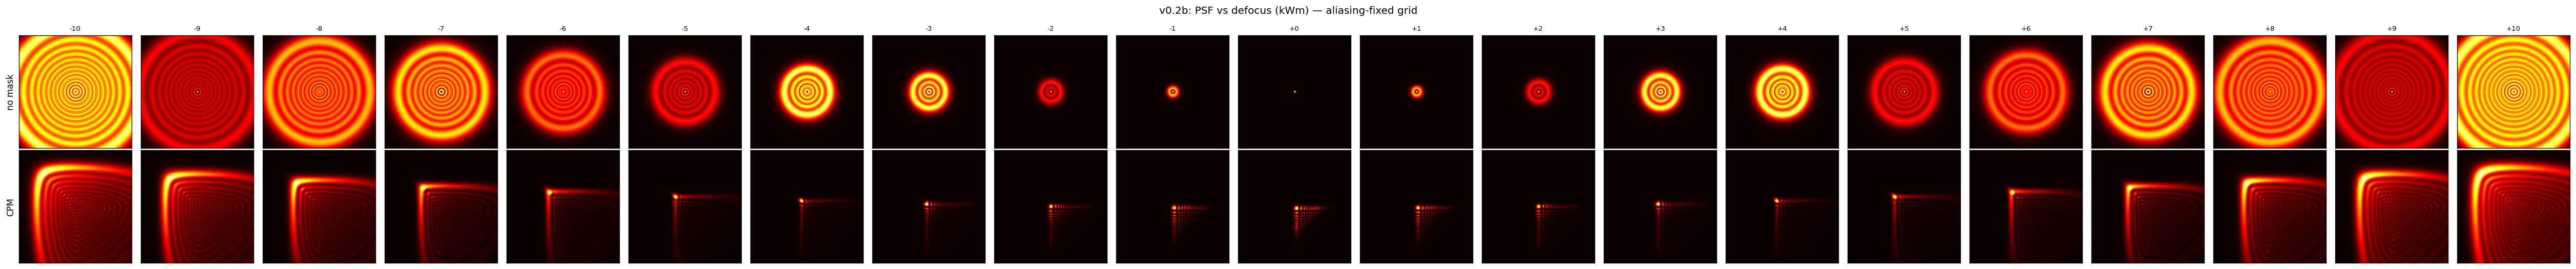
\includegraphics[width=0.95\textwidth]{fig_psf_comparison_grid.png}
\caption{kWm=$-10\sim+10$におけるPSF(上段: no mask、下段: CPM)。CPMはデフォーカスしても形状をほぼ保つ。}
\label{fig:psf}
\end{figure}

\subsection{Wienerデコンボリューションによる復元(定性評価)}
合焦時に測定した単一のPSFを固定カーネルとしてWiener復元した結果を、合成チャープ画像(図\ref{fig:edof_demo})と点光源(図\ref{fig:point_source})の2種類のテスト画像で確認した。

\begin{figure}[H]
\centering
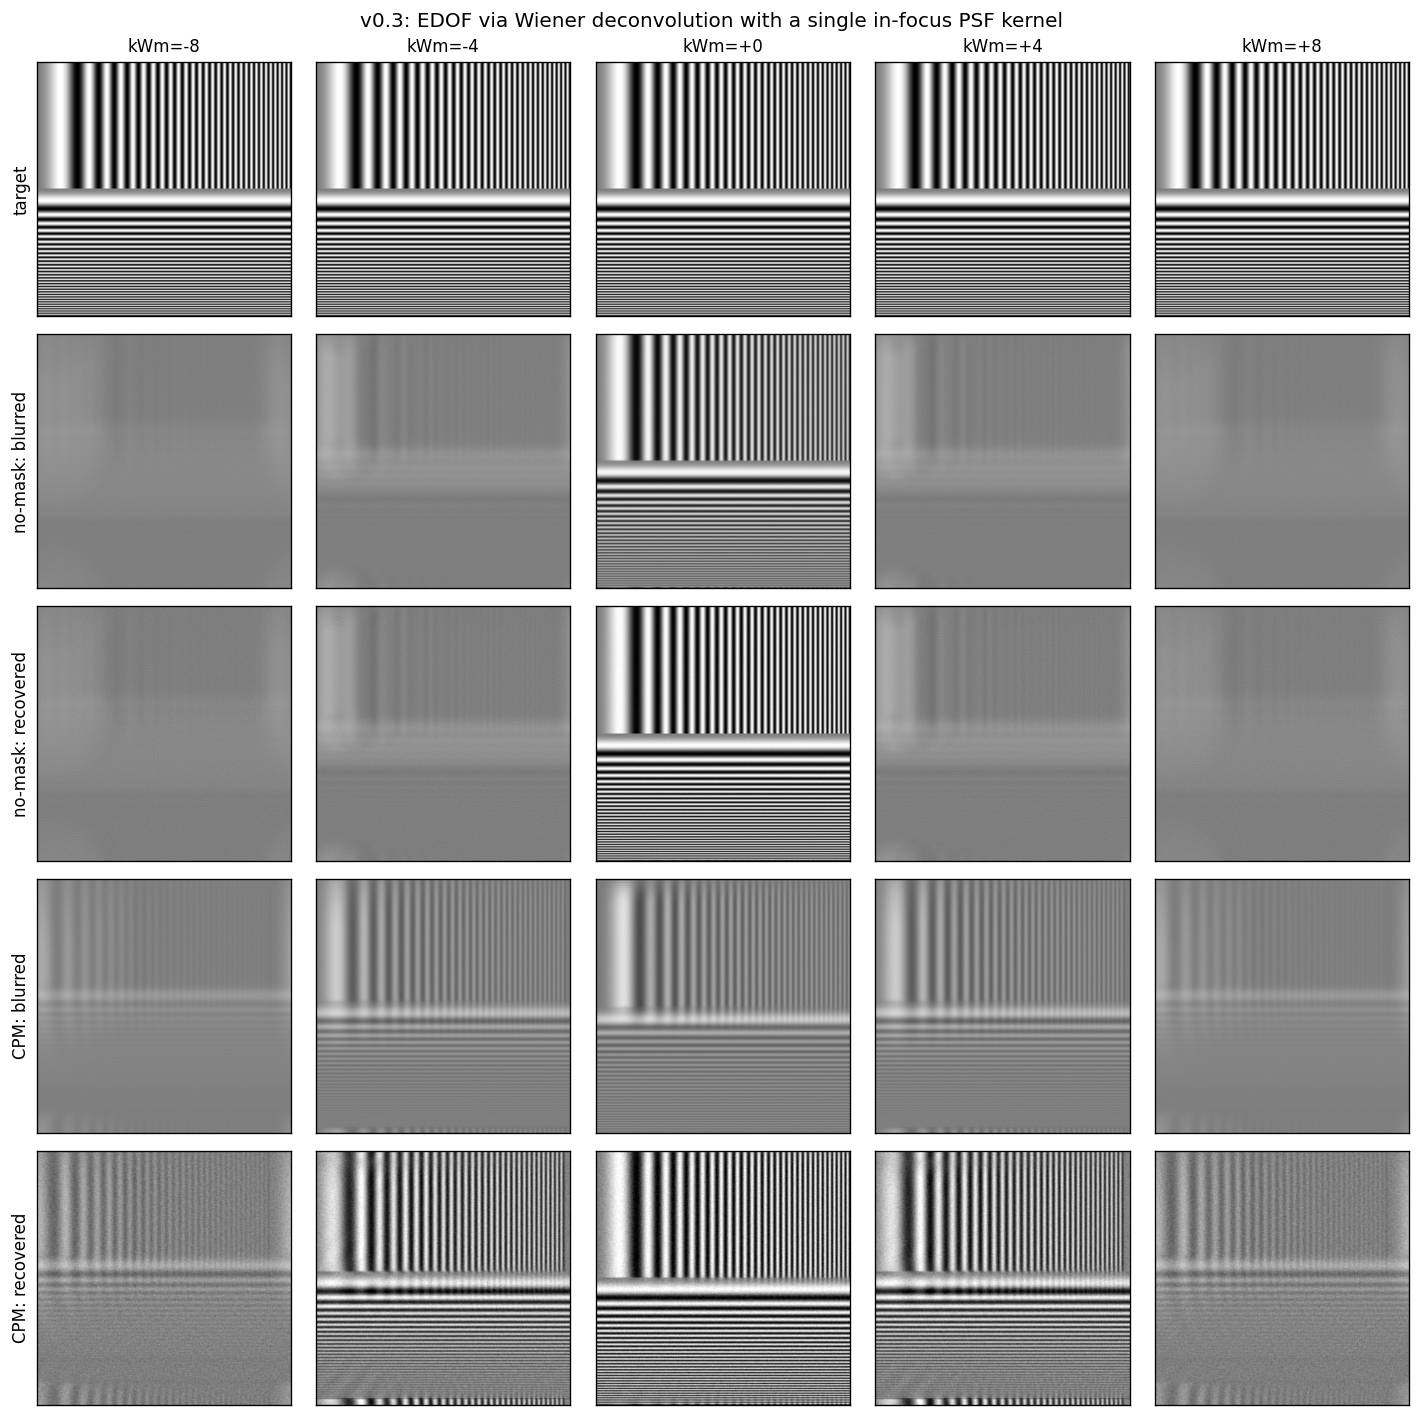
\includegraphics[width=\textwidth]{fig_edof_demo.png}
\caption{合成チャープ画像を用いたWiener復元例(kWm=$-8,-4,0,+4,+8$)。上から順に正解画像、no maskのぼけ画像・復元画像、CPMのぼけ画像・復元画像。}
\label{fig:edof_demo}
\end{figure}

チャープ画像(図\ref{fig:edof_demo})では、$|kWm|\le4$の範囲でCPMの復元結果がno maskよりも縞模様を明瞭に保っており、$|kWm|=8$でもCPMは粗い縞の情報をわずかに残すのに対し、no maskの復元像はすでに一様なグレーへ潰れている。

\begin{figure}[H]
\centering
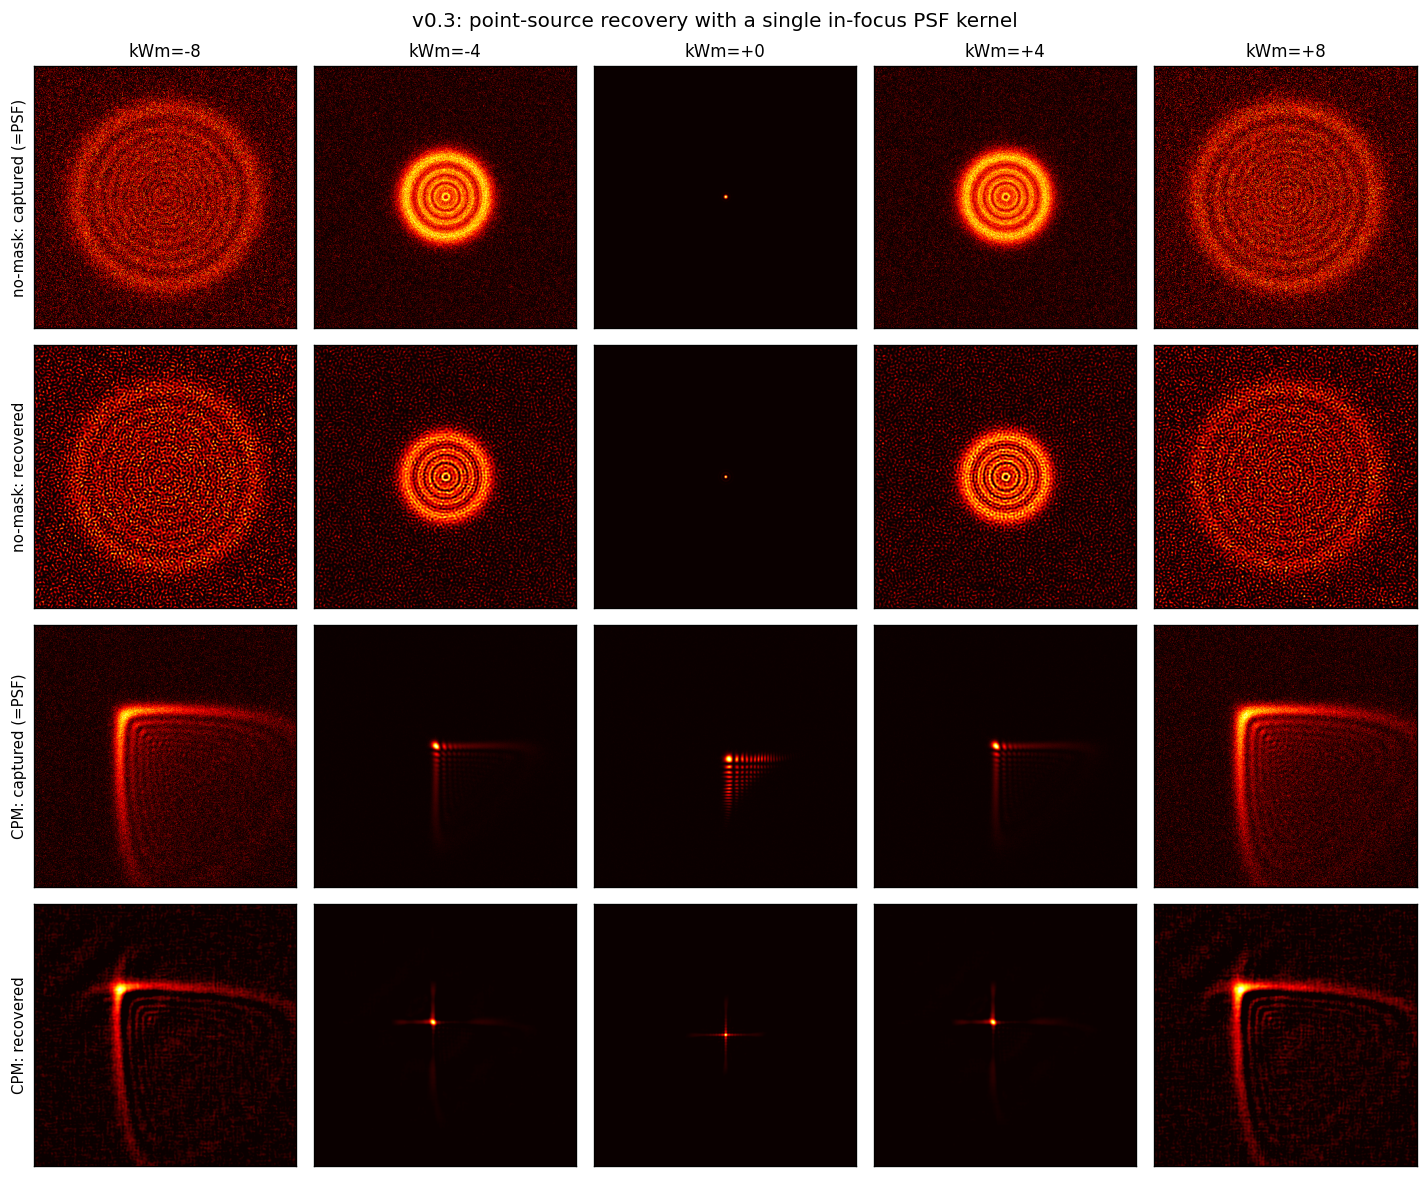
\includegraphics[width=\textwidth]{fig_point_source_demo.png}
\caption{点光源(=PSFそのもの)を撮影画像として用いたWiener復元例(kWm=$-8,-4,0,+4,+8$)。上から順にno maskの撮影画像・復元画像、CPMの撮影画像・復元画像。}
\label{fig:point_source}
\end{figure}

点光源テスト(図\ref{fig:point_source})でも同様の傾向が見られ、$kWm=\pm4$でCPMの復元像は鋭い十字状のピークを保つが、no maskの復元像はぼやけたリングのままであり、視覚的にもCPMのEDOF効果を確認できる。ただし$kWm=\pm8$まで離焦するとCPM自身の不変性も崩れ、両者とも実質的に復元が破綻する。

\subsection{定量評価(PSNR・シャープネス)}

\begin{figure}[H]
\centering
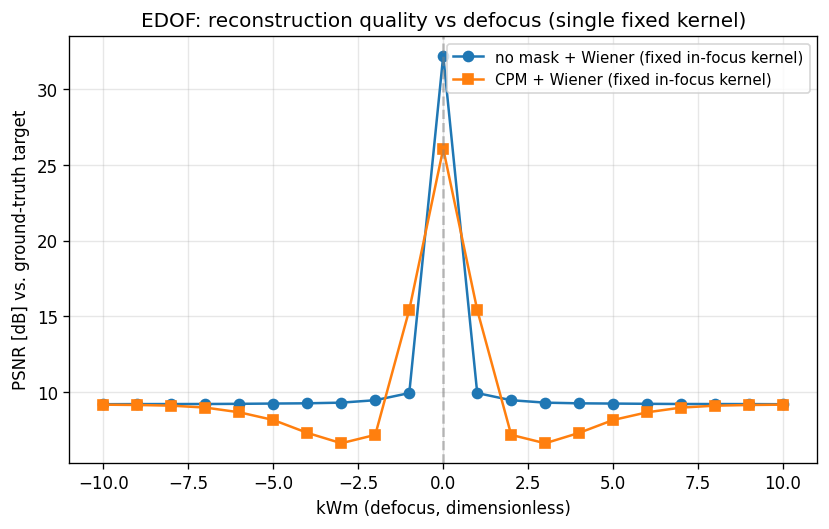
\includegraphics[width=0.75\textwidth]{fig_psnr.png}
\caption{合成チャープ画像のPSNR vs デフォーカス量(青: no mask、橙: CPM)。}
\label{fig:psnr}
\end{figure}

チャープ画像のPSNR(図\ref{fig:psnr})は非単調な挙動を示した。合焦点$kWm=0$では、CPM自身のPSF形状に起因する設計上のトレードオフにより、no maskが大きく優位である($\sim32\,\text{dB}$ vs $\sim26\,\text{dB}$)。一方$kWm=\pm1$では、no maskの復元がほぼ完全に失敗するのに対しCPMは依然情報を保っており、CPMが$+5.5\,\text{dB}$優位に転じる。$1<|kWm|\le5$では再びno maskがわずかに優位に戻り、$|kWm|\approx10$では両者とも同程度の低い値に収束する。

\begin{figure}[H]
\centering
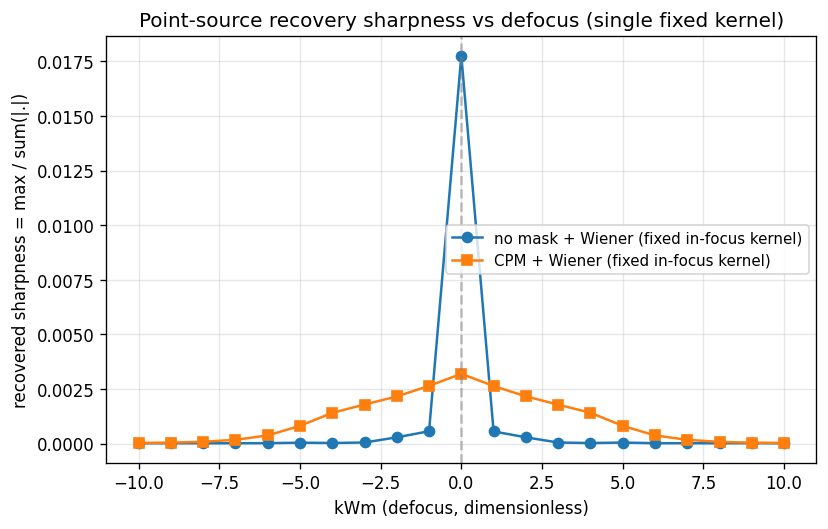
\includegraphics[width=0.75\textwidth]{fig_sharpness.png}
\caption{点光源+シャープネスによるEDOF評価(青: no mask、橙: CPM)。}
\label{fig:sharpness}
\end{figure}

一方、点光源のシャープネス(図\ref{fig:sharpness})は単調な傾向を示した。合焦点付近($|kWm|\le1$)ではno maskの方がシャープに復元できる(CPM自身のPSFが十字型に広がる設計上のトレードオフのため)が、それ以外の$|kWm|\ge2$の全域でCPMが一貫して優位(平均で約16倍のシャープネス)であった。PSNRとは異なりシャープネスが単調な結果になった理由は、後述の通り評価指標そのものの性質に起因すると考えられる。

\subsection{結果のまとめ}
\begin{table}[H]
\centering
\small
\caption{3方向の検証結果まとめ}
\label{tab:summary}
\begin{tabular}{@{}p{4.2cm}p{9.3cm}@{}}
\toprule
検証方法 & 結果 \\
\midrule
NCC(PSF形状不変性) & $|kWm|\ge 6$でもCPMが明確に優位(0.48 vs 0.04) \\
チャープ画像+PSNR & 非単調。合焦点($kWm=0$)はno maskが優位だが、$kWm=\pm1$でCPMが$+5.5\,\text{dB}$優位に転じ、$1<|kWm|\le5$では再びno mask優位に戻る \\
点光源+シャープネス & 単調。$|kWm|\ge 2$の全域でCPMが一貫して優位(平均約16倍) \\
\bottomrule
\end{tabular}
\end{table}

% =====================================================================
\section{得られた知見}
% =====================================================================
\begin{itemize}[topsep=2pt, itemsep=2pt]
  \item CPMは、PSF形状不変性(NCC)・点光源復元(シャープネス)の両指標で、no maskより広いデフォーカス範囲で明確に優位であることを確認した。report\_chang.pdf相当のEDOFはおおむね再現できたと判断している。
  \item 一方、画素単位の誤差(PSNR)は非単調な結果を示した。これはno maskが「無難に平坦な出力へ失敗する」のに対し、CPMは「構造化された誤り」を犯しうるためであり、\textbf{単一の評価指標だけで判断すると結論を誤りうる}ことが最大の教訓である。
  \item CPMの不変性には有限範囲があり($|kWm|\lesssim 6\sim8$)、これはreport\_chang.pdfが報告する実測範囲($\pm30\sim50\,\mu\text{m}$)と定性的に整合する。
\end{itemize}

% =====================================================================
\section{今後の予定}
% =====================================================================
次はv0.4として、本研究の独自性である斜め照明70〜80°への拡張に進む。これまでの前提(垂直入射・回転対称な離焦位相)が崩れることで、CPMの不変性やPSFの形状にどう影響するかを検証する。また、\texttt{PUPIL\_HALF\_WIDTH}や$kWm$を物理単位($\mu$m)へ対応づける作業も、実スケールでの評価に必要な課題として残っている。

\printbibliography

\end{document}
